\documentclass{beamer}

\mode<presentation>{
\usetheme{PaloAlto}
%\usetheme{Berlin}
\usecolortheme{default}
\usefonttheme{professionalfonts}
}

\usepackage[utf8]{inputenc}
\usepackage{babel}
\usepackage{graphicx}
\usepackage{booktabs}
\usepackage{svg}
\usepackage{url}
\usepackage{appendixnumberbeamer}
\usepackage{subfigure}
\usepackage{hyperref}

\usepackage{physics}
\graphicspath{{figs}}
%\usepackage{relsize}
\usepackage{amsmath}
\usepackage{commath}
\usepackage{xfrac}
\usepackage{xcolor}

\title{The Hubbard Model in Low Dimensions}
\author{Christoph Gäntgen and Ulli Pohl}
\institute[]{Physikalisches Institut\\
	Rheinische Friedrich-Wilhelms-Universität Bonn}
\date{March 31st 2020}


\makeatletter
\setbeamertemplate{sidebar \beamer@sidebarside}%{sidebar theme}
{
	\beamer@tempdim=\beamer@sidebarwidth%
	\advance\beamer@tempdim by -6pt%
	\insertverticalnavigation{\beamer@sidebarwidth}%
	\vfill
	\ifx\beamer@sidebarside\beamer@lefttext%
	\else%
	\usebeamercolor{normal text}%
	\llap{\usebeamertemplate***{navigation symbols}\hskip0.1cm}%
	\vskip2pt%
	\fi%
}%
\makeatother
%\setbeamersize{sidebar width left = 3.6em}

\begin{document}

\begin{frame}
\titlepage
\end{frame}

\begin{frame}
\frametitle{Inhalt}
\tableofcontents
\end{frame}

\section{Motivation}
\begin{frame}
\frametitle{Motivation}
\begin{itemize}
	\item Simplified model - still exhibits interesting physics 
	\item Examples: metal-insulator transition, antiferromagnetism and superconductivity
	\item Exact diagonalization is too time-/storageexpensive $\rightarrow$ Monte Carlo Integration
\end{itemize}
\end{frame}

\section{Theoretical background}
\subsection{Hubbard model}
\begin{frame}
\frametitle{Hubbard model - A simplified model}
\begin{figure}[h]
	\centering
	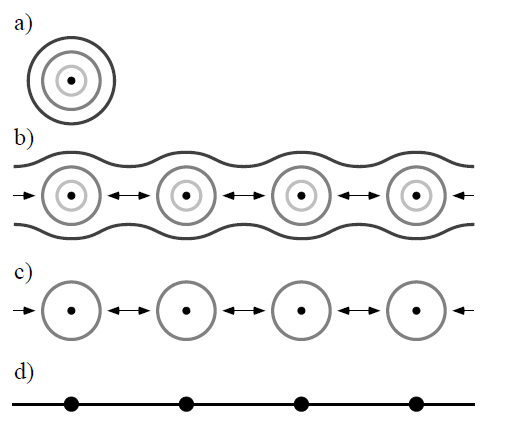
\includegraphics[width=0.6\linewidth]{pic0}
	\caption{From valence electrons and bound electrons to the Hubbard simplification}
	\label{fig:pic0}
\end{figure}
\end{frame}

\begin{frame}
	\frametitle{Hubbard model - 2}
	\begin{figure}[h]
		\centering
		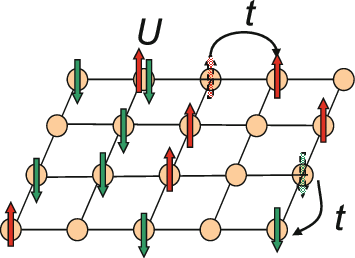
\includegraphics[width=0.4\linewidth]{pic2}
		\caption{Illustration of the model on a 2D lattice}
		\label{fig:pic2}
	\end{figure}
	\begin{equation*}\label{Hubbard_standard}
	H = -t\sum_{\langle ij\rangle,\sigma}\left( c_{i\sigma}^\dag c_{j\sigma} + c_{j\sigma}^\dag c_{i\sigma}\right) + U \sum_{i}n_{i\uparrow}n_{i\downarrow}
	\end{equation*}
\end{frame}

\begin{frame}
\frametitle{Hubbard model - Fock space}
\begin{itemize}
\item Fock space containing all many body states of the Hamiltonian
\item Example 1 site lattice: \[ \ket{0},\; \ket{\uparrow},\; \ket{\downarrow}\; \text{oder} \; \ket{\uparrow\downarrow}\]
\item For $L$ lattice sites $ 4^L $ possible states, but
\end{itemize}
\[ H=\left( \begin{array}{ccc}
H_{N=0}  & 0 & 0\\
0 & H_{N=1} & 0\\
0 & 0 & H_{N=2}\\
\end{array}\right)  \]
$ \Rightarrow $ Basis splits up

\end{frame}

%\begin{frame}
%\frametitle{Impuls-Basis}
%Diagonalisierter hopping-Term:
%\[ H_0 = \sum_{\boldsymbol{k} \sigma} \epsilon_{\boldsymbol{k}} c_{\boldsymbol{k}\sigma}^\dag c_{\boldsymbol{k}\sigma} \]
%Fourier-transformierte Operatoren:
%\[ c_{\boldsymbol{k}\sigma} = \frac{1}{\sqrt{N}}\sum_{j} e^{i\boldsymbol{k}\boldsymbol{R}_j} c_{j\sigma}, \qquad c_{\boldsymbol{k}\sigma}^\dagger = \frac{1}{\sqrt{N}}\sum_{j} e^{-i\boldsymbol{k}\boldsymbol{R}_j} c_{j\sigma}^\dagger \]
%Impulszustand:
%\[ \ket{a(k)} = \frac{1}{\sqrt{N_a}}\sum_{r=0}^{N-1}e^{-ikr}T^r\ket{a} \]
%\end{frame}

\subsection{Correlation functions}
\begin{frame}
\frametitle{Correlation functions}
\begin{itemize}
	\item Canonical ensemble
	\item Partition function 
	\begin{equation*}
	Z := \text{Tr}(\text{e}^{-\beta H}) = \sum_{n}^{}\text{e}^{-\beta E_n} \label{partition}
	\end{equation*}
\item Energy expectation value
\begin{equation}
\langle{E}\rangle = \frac{1}{Z}\text{Tr} (H\text{e}^{-\beta H}) =\frac{1}{Z} \sum_{n}^{} E_n\text{e}^{-\beta E_n} \label{energy}
\end{equation}	
\end{itemize}
%Die Selbstkonsistenz-Bedingung muss erfüllt sein
\end{frame}
\subsection[Analytic solutions]{Analytic solution for small lattices}
\begin{frame}
\frametitle{Analytic solution of the model for small lattices}
\begin{itemize}
\item For 1 (2) lattice sites only 4(16) states in Fock space
\item can find expressions for correlaors analytically
\end{itemize}
\end{frame}



\begin{frame}
\frametitle{Solving the 1 site model}

\begin{figure}[h]
	\centering
	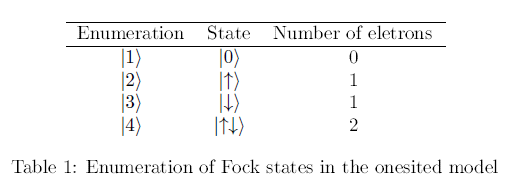
\includegraphics[width=0.7\linewidth]{states}
	\label{fig:states1}
\end{figure}
\begin{equation*}
\langle i|H|j\rangle=
\begin{pmatrix}
0 & 0 & 0&0\\
0 & -\frac{U}{2} & 0&0\\
0 & 0 & -\frac{U}{2}&0\\
0 & 0 & 0&0
\end{pmatrix}
\end{equation*}
\begin{equation}
Z_{1}= 2 (1+\text{e}^{\beta U/2})
\label{partition1}
\end{equation}
\end{frame}


\section{Methods}

\subsection{Metropolis algorithm for the 1D Hubbard model}
\begin{frame}
\frametitle{Metropolis algorithm}
Basisdarstellung:
\[ \ket{L_\uparrow,L-1_\uparrow,\dots,2_\uparrow,1_\uparrow,L_\downarrow,L-1_\downarrow,\dots,2_\downarrow,1_\downarrow} \]
Beispiel:
\[ \ket{\downarrow_1,-_2,\uparrow\downarrow_3}\;\rightarrow \; c^\dagger_{3\uparrow}c^\dagger_{3\downarrow}c^\dagger_{1\downarrow}\ket{0} = \ket{1, 0, 0, 1, 0 , 1} = \ket{37} \]\pause
\begin{block}{Wichtig!}
Fermionen $ \Rightarrow $ Vorzeichenwechsel beachten!
\[ c^\dagger_{1\uparrow}\ket{37} =  c^\dagger_{1\uparrow}c^\dagger_{3\uparrow}c^\dagger_{3\downarrow}c^\dagger_{1\downarrow}\ket{0}=-c^\dagger_{3\uparrow}c^\dagger_{1\uparrow}c^\dagger_{3\downarrow}c^\dagger_{1\downarrow}\ket{0}=-\ket{45}\]
\end{block}
\end{frame}

\begin{frame}
\frametitle{Metropolis algorithm - 2}
\begin{block}{Impulszustand}
\[ \ket{a(k)} = \frac{1}{\sqrt{N_a}}\sum_{r=0}^{N-1}e^{-ikr}T^r\ket{a} \]
\end{block}
\[ T^m\ket{a(k)} = e^{ikm}\frac{1}{\sqrt{N_a}}\sum_{r=0}^{N-1}e^{-ik(r+m)}T^{r+m}\ket{a}=e^{ikm}\ket{a(k)} \]
\[ \bra{a(k)}O\ket{b(k)} = \pm\sqrt{\frac{N_a}{N_b}}e^{ikm} \bra{T^ma}O\ket{b} \]
\end{frame}
\subsection{Monte Carlo Integration}
\begin{frame}
\frametitle{Hubbard-Stratonovich transformation}
\begin{block}{Problem}
Der Operator ist häufig zu groß um als Matrix gespeichert zu werden
\end{block}
Beispiel:
\[ H\;\rightarrow\; \mathtt{cx\_vec\: Hamilton(uvec\: Basis,\:cx\_vec\: Psi)}\]


\[ \ket{\psi_{out}} = \sum_{n,m}B^{-1}_{out}\ket{m}\bra{m}OB_{in}\ket{n}\bra{n}\ket{\psi_{in}} \]
\end{frame}

\begin{frame}
\frametitle{Integration}
\begin{enumerate}
	\item suche Grundzustand (in allen k-Unterräumen)
	\begin{itemize}
		\item für jeden k-Unterraum wird ein Lanczos-Verfahren benötigt um den jeweils kleinsten Eigenwert zu finden
	\end{itemize}
\end{enumerate}
\vbox{}\vbox{}\vbox{}\vbox{}\vbox{}\vbox{}\vbox{}\vbox{}\vbox{}\vbox{}\vbox{}\vbox{}
\end{frame}



\begin{frame}
\frametitle{Vorgehen beim erstellen der Spektralfunktion}
\begin{enumerate}
\item suche Grundzustand (in allen k-Unterräumen)
\begin{itemize}
	\item für jeden k-Unterraum wird ein Lanczos-Verfahren benötigt um den jeweils kleinsten Eigenwert zu finden
	\item für den Grundzustand ein zusätzliches Lanczos-Verfahren um den Vektor in die korrekte Basis zu transformieren\pause
	\item zur Wiederverwendung abspeichern\pause
\end{itemize}
\item der passende Vernichtungsoperator wird auf den Grundzustand angewandt um den Startzustand zu erhalten\pause
\item ein Lanczos-Verfahren wird mit dem Startvektor begonnen um die Green'sche Funktion zu erhalten\pause
\item die Spektralfunktion wird aus der Green'schen Funktion bestimmt\pause
\item die Schritte 2-4 werden auch für den Erzeugungsoperator wiederholt und die Spektralfunktionen werden addiert
\end{enumerate}
\end{frame}

\section{Results}
\subsection{Partition function...energy expectation oder so}
%\begin{frame}
%\frametitle{Konvergenz zur analytischen Lösung}
%\begin{figure}[h]
%	\centering
%	\includegraphics[width=0.8\linewidth]{Praesentation-Bilder/konvergenz}
%	\caption{Grundzustandsenergie pro Gitterplatz für U=t=1}
%	\label{fig:konvergenz}
%\end{figure}
%
%\end{frame}





\section[Conclusion and Outlook]{Conclusion and Outlook}
\begin{frame}
\frametitle{Conclusion}
\begin{block}{Successes}
\begin{itemize}
\item 1- and 2-site partition function matching (energy, correlator?)
\end{itemize}
\end{block}

\begin{block}{Outlook}
	\begin{itemize}
		\item Optimize in precision
		\item Optimize in computing time
		\item Higher dimensional model
		\item Grand-canonical ensemble (pairwise creation of electrons allowed)
	\end{itemize}
\end{block}
\end{frame}

\appendix

\begin{thebibliography}{}
\begin{frame}
\frametitle{References}	
	\bibitem{luu}
	Thomas Luu 2017
	\textit{Fermions and Computers}
	
	\bibitem{lieb}
	E. Lieb, F. Wu 2003
	\textit{The one-dimensional Hubbard model: A Reminiscence}
	
	\bibitem{tasaki} 
	H. Tasaki 1998
	\textit{The Hubbard model - An Introduction and selected rigorous Results}
	
	\bibitem{jafari}
	Seyed A. Jafari 2008
	\textit{Introduction to Hubbard Model and Exact Diagonalization}	
\end{frame}	
\begin{frame}
\frametitle{References - 2}
\bibitem{gabrielsson}
Anders F. Gabrielsson 2011
\textit{Quantum Monte Carlo Simulations of
	the Half-filled Hubbard Model}

\bibitem{Hubbard}
M. Machida et al. \textit{High Performance LOBPCG Method for Solving Multiple Eigenvalues of Hubbard Model: Efficiency of Communication Avoiding Neumann Expansion Preconditioner}
\bibitem{Hubbard2}
\textit{http://atomcool.rice.edu/research/3d-lattice/}
\end{frame}
\end{thebibliography}




\end{document}